\documentclass{beamer}

\usepackage[utf8]{inputenc}
\usepackage{default}


\usepackage{multirow} %for aligning stuff in tables

\usepackage{bbding} %for the smiley face

\usepackage{calc} %calculate spacing \widthof

%tikz stuff
\usepackage{tikzsymbols}
\usepackage{tikz}
\usetikzlibrary{fit,arrows,positioning}

  % Keys to support piece-wise uncovering of elements in TikZ pictures:
  % \node[visible on=<2->](foo){Foo}
  % \node[visible on=<{2,4}>](bar){Bar}   % put braces around comma expressions
  %
  % Internally works by setting opacity=0 when invisible, which has the 
  % adavantage (compared to \node<2->(foo){Foo} that the node is always there, hence
  % always consumes space plus that coordinate (foo) is always available.
  %
  % The actual command that implements the invisibility can be overriden
  % by altering the style invisible. For instance \tikzsset{invisible/.style={opacity=0.2}}
  % would dim the "invisible" parts. Alternatively, the color might be set to white, if the
  % output driver does not support transparencies (e.g., PS) 
  %
  \tikzset{
    invisible/.style={opacity=0},
    visible on/.style={alt={#1{}{invisible}}},
    alt/.code args={<#1>#2#3}{%
      \alt<#1>{\pgfkeysalso{#2}}{\pgfkeysalso{#3}} % \pgfkeysalso doesn't change the path
    },
  }
  \tikzset{
    dimmed/.style={opacity=0.2},
    dimmed on/.style={alt={#1{dimmed}{}}},
    alt/.code args={<#1>#2#3}{%
      \alt<#1>{\pgfkeysalso{#2}}{\pgfkeysalso{#3}} % \pgfkeysalso doesn't change the path
    },
  }
\tikzset{
    %Define standard arrow tip
    >=stealth',
    %Define style for boxes
    peer/.style={
           rectangle,
           rounded corners,
           draw=black, thin,
           text width=3.5em,
           minimum height=2em,
           text centered},
    node/.style={
           rectangle,
           rounded corners,
           draw=black, 
           text width=4.5em,
           minimum height=2em,
           text centered,
           fill={rgb:black,1;white,3}},
    chunk/.style={
           rectangle,
           rounded corners,
           draw=black, 
           text width=2.5em,
           minimum height=1em,
           text centered,
           fill=block title bg},
    % Define arrow style
    point/.style={
           ->,
           thick,
           shorten <=2pt,
           shorten >=2pt,}
every node/.style={align=center}           
}

\newcommand{\wholeslide}[2][]{
\begin{frame}{#1}
% \transboxout<1>[duration=0.5]
\setbeamercolor{bgcolor}{fg=black,bg=white}
\begin{tikzpicture}[overlay, remember picture]
\node[anchor=center] at (current page.center) {
  \begin{beamercolorbox}[center]{bgcolor}
     #2
  \end{beamercolorbox}};
\end{tikzpicture}

\end{frame}
}

\newcommand{\blankslide}[2][]{
\begin{frame}[plain]{#1}
% \transboxout<1>[duration=0.5]
\setbeamercolor{bgcolor}{fg=black,bg=white}
\begin{tikzpicture}[overlay, remember picture]
\node[anchor=center] at (current page.center) {
  \begin{beamercolorbox}[center]{bgcolor}
     #2
  \end{beamercolorbox}};
\end{tikzpicture}

\end{frame}
}

\newenvironment<>{varblock}[2][.9\textwidth]{%
  \setlength{\textwidth}{#1}
  \begin{actionenv}#3%
    \def\insertblocktitle{#2}%
    \par%
    \usebeamertemplate{block begin}}
  {\par%
    \usebeamertemplate{block end}%
  \end{actionenv}}

\newlength{\mywidth}
\newcommand{\blockslide}[3][]{
\settowidth{\mywidth}{#3}
\begin{frame}[c]{#1}
\begin{center}
\begin{minipage}{1.1\mywidth}
 \begin{varblock}[1.1\mywidth]{#2}
  #3
 \end{varblock}
\end{minipage}
\end{center}
\end{frame}
}

\mode<presentation>{
\usetheme{Warsaw}\usecolortheme{crane}
\setbeamertemplate{items}[square]
\setbeamertemplate{section in toc}[square]
\setbeamertemplate{subsection in toc}[square]
% \setbeamertemplate{subsection in toc}[subsections numbered]
\setbeamertemplate{subsubsection in toc}[square]
% \setbeamercolor{items}{fg=black,bg=yellow}
\usebeamercolor{block title}
\definecolor{block title bg}{named}{bg}
\setbeamercolor{item projected}{fg=black,bg=block title bg}
\setbeamercolor{itemize item}{fg=block title bg,bg=block title bg}
}







\title{Towards web3 infrastructure}
\author{Viktor Trón}

\AtBeginSection[]
{
\begin{frame}<beamer>
\frametitle{Outline}
\tableofcontents[currentsection,sectionstyle=show/shaded,subsectionstyle=show/show/hide,subsubsectionstyle=show/show/show/hide]
\end{frame}
}

\begin{document}

\begin{frame}
 \titlepage
\end{frame}

\begin{frame}
\begin{block}{}
\begin{itemize}
\item peer to peer technologies with incentives
\item base layer infrastructure for the third web
\item decentralised dev stack
\end{itemize}
\end{block}
\end{frame}

\begin{frame}[plain,c]
\begin{center}
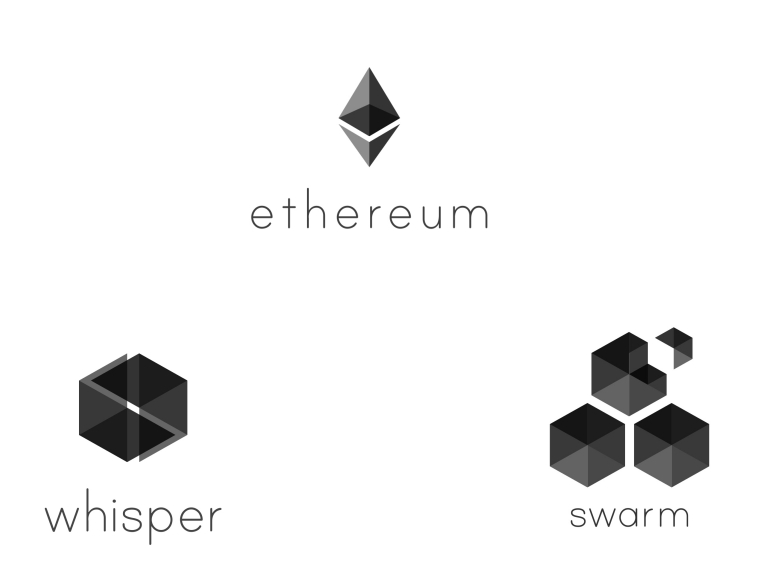
\includegraphics[width=0.8\textwidth]{ecosystem0.jpg}
\end{center}
\end{frame}

\begin{frame}
 \tableofcontents[subsectionstyle=shaded/shaded,subsubsectionstyle=hide/hide]
\end{frame}


\begin{frame}[t]{\alt<5->{it's chunks all the way down...}{Chunks}}
% \begin{overlayarea}{⟨area width⟩}{⟨area height⟩}
%   ⟨environment contents⟩
% \end{overlayarea}
\begin{overlayarea}{\textwidth}{10cm}
under the hood swarm does not deal in files but in \emph{chunks.}

\begin{itemize}
 \item<2-> all data is broken into pieces of size 4kB: ``chunks".
 \item<4-> chunks are hashed and the hash is used as their ID/address.
 \item<5-> chunk hashes are also packaged into 4kB chunks...
\end{itemize}

\begin{onlyenv}<1-2>
 \begin{center}
  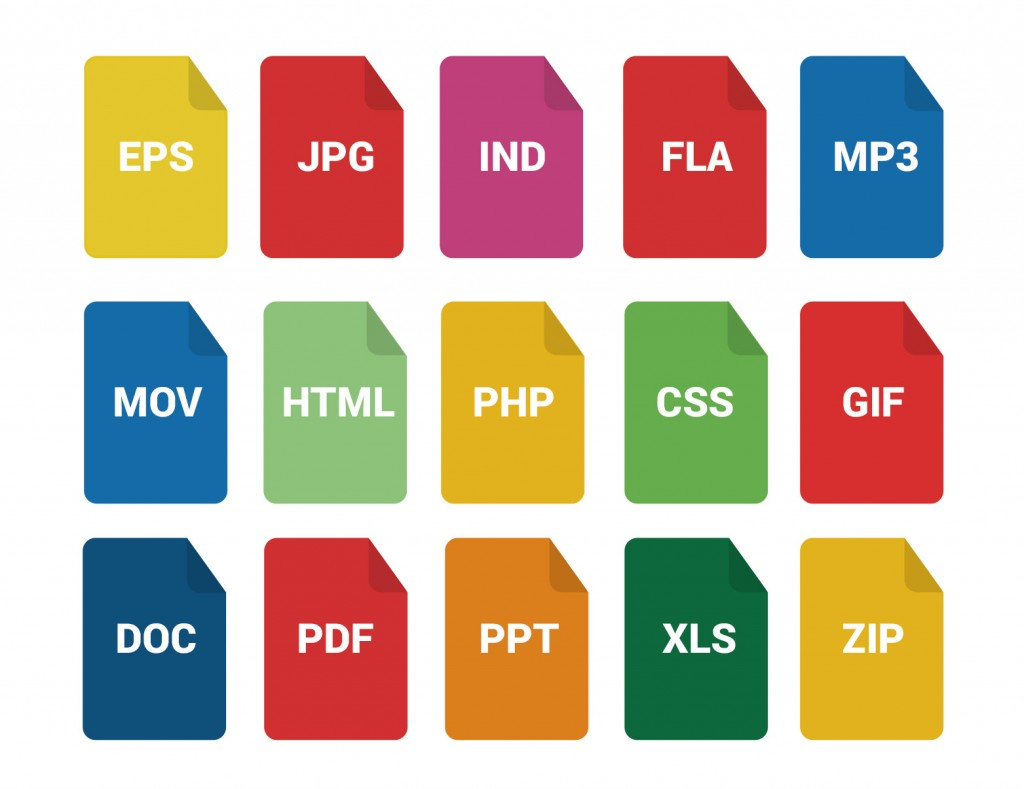
\includegraphics[width=0.4\textwidth]{devcon-files.jpg}
  \transdissolve<3>
 \end{center}
\end{onlyenv}

 \begin{center}
  \begin{tikzpicture}
   \node[chunk,visible on=<3>] at (0,0) (achunk){};
   \node[visible on=<3>] at (-1.8,0) (labeltext){A ``chunk:"};
   \node[chunk,visible on=<3->] at (-4,-3) (a){};
   </3-></3>   \node[chunk,visible on=<3->] at (-2,-3) (b){};
   \node[chunk,visible on=<3->] at (0,-3) (c){};
   \node[chunk,visible on=<3->] at (2,-3) (d){};
   \node[chunk,visible on=<3->] at (4,-3) (e){};

   \node at (-4.2,-1.3) (dummy1) {};
   \node at (4.2,-1.7) (dummy2) {};
   \node[chunk,fit=(dummy1)(dummy2),visible on=<5>]{};

   \node[scale=0.8,draw,visible on=<4-5>] at (-4,-1.5) (ha){$h_1$}
     (a.north) edge[-,visible on=<4>] (ha.south);
   \node[scale=0.8,draw,visible on=<4-5>] at (-2,-1.5) (hb){$h_2$}
     (b.north) edge[-,visible on=<4>] (hb.south);
   \node[scale=0.8,draw,visible on=<4-5>] at (0,-1.5) (hc){$h_3$}
     (c.north) edge[-,visible on=<4>] (hc.south);
   \node[scale=0.8,draw,visible on=<4-5>] at (2,-1.5) (hd){$h_4$}
     (d.north) edge[-,visible on=<4>] (hd.south);
   \node[scale=0.8,draw,visible on=<4-5>] at (4,-1.5) (he){$h_5$}
     (e.north) edge[-,visible on=<4>] (he.south);

   \node[chunk,visible on=<6>] at (0,-1.5) {};
     \end{tikzpicture}

 \end{center}
\end{overlayarea}
\end{frame}

\begin{frame}
\begin{overlayarea}{\textwidth}{10cm}

 \begin{columns}[T]
  \begin{column}{0.5\textwidth}
  chunks are assembled in a \textbf{Merkle Tree}.
  \small
    \begin{itemize}
     \item<1->{files are retrievable using a single 32byte hash}
     \item<1->{built-in integrity protection and random access}
     \item<2->{merkle-proofs enable proof-of-custody schemes}
     \item<3->{traversible using ASCII charactes due to branching factor of 128}
    \end{itemize}

  \end{column}
  \begin{column}{0.5\textwidth}
   \only<1-2>{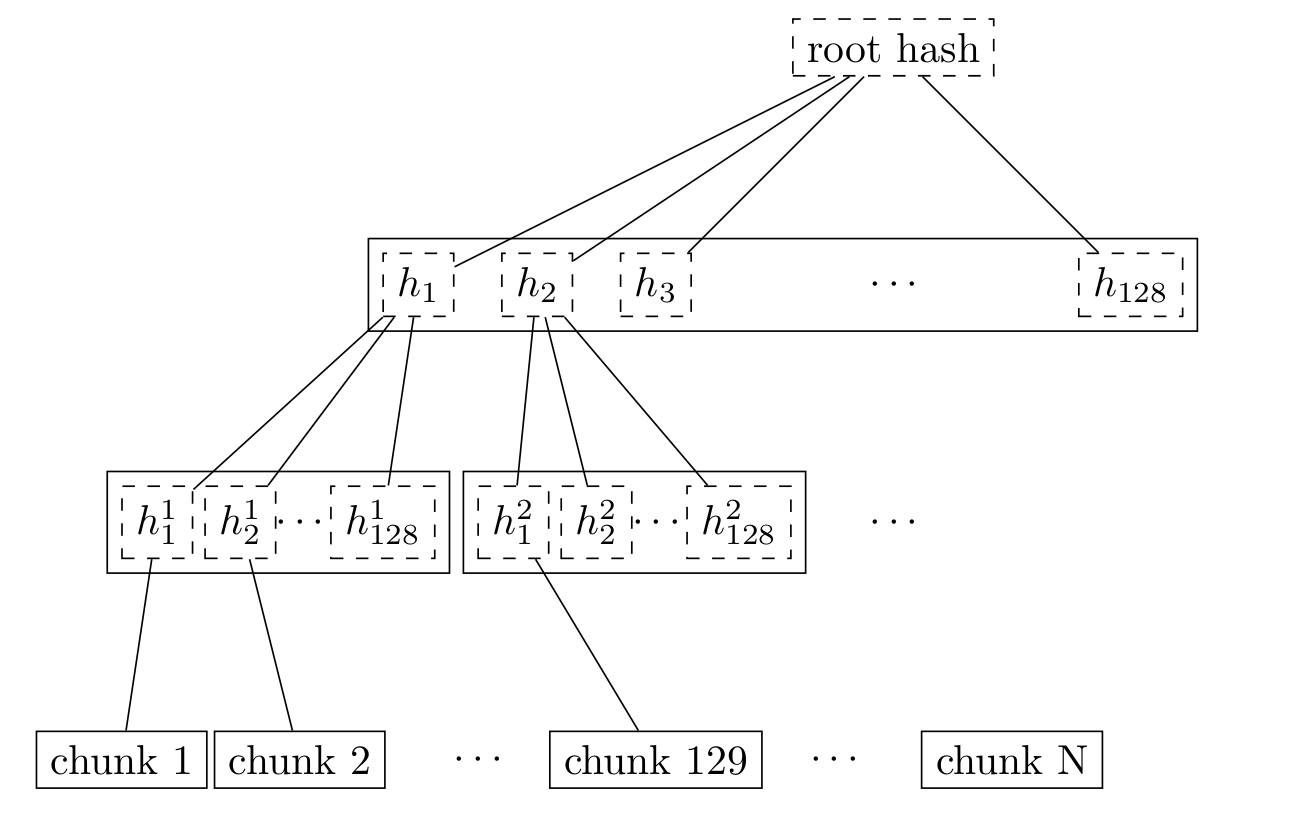
\includegraphics[width=6cm]{devcon-merkle-tree.png}}
   \only<3>{
   \begin{tikzpicture}
    \node[scale=0.4] {
    \documentclass[border=2pt,draw]{standalone}
\usepackage{tikz}
\usetikzlibrary{fit}
\begin{document}

\tikzset{
level/.style={
  sibling distance={(width("$H^126$")+4pt)},
  level distance=15mm,
  line width=.5pt,
},
mtnode/.style={
  minimum width={width("$H^126$")+2pt},
  minimum height={.7cm},
  inner sep=2pt,
  outer sep=2pt,
  rectangle,
  rounded corners=1pt,
  draw,
},
% edge from parent/.style={draw=none},
mtedge/.style={grow=down,draw=none,<-, edge from parent/.style={draw}},
link/.style={draw=none, edge from parent/.style={draw=none}},
mtedgeadj/.style={mtedge, shorten >=10pt  },
mpedge/.style={mtedge, line width=.7pt,densely dashed},
ellip/.style={draw,loosely dotted, shorten >=5mm, thick,<-, edge from parent/.style={draw}},
bubble/.style={minimum height={1cm}, draw=none, align=center},
data/.style={mtnode, fill=gray!50},
mppath/.style={mtnode,dashed,line width=.7pt,fill=gray!30},
mpext/.style={mtnode,line width=.7pt,fill=gray!40},
mpdata/.style={data,line width=.7pt,fill=gray!70},
mpdataext/.style={data,line width=.7pt,fill=gray!80},
}

\begin{tikzpicture}
                  % level 7
\node[mtnode] (root) {$H^7_0$}
                  % level 6
  child[<-,grow=right,level distance=3cm] { node[bubble] (ash) {root-hash}  }
  % child[link,grow=left,level distance=5cm] { node[bubble] (ash) {audit secret}  }
  child { node[mppath] (6-0) {$H^6_0$}   % 0
                  % level 5
    child { node[mppath] (5-0) {$H^5_0$}          % 0
      % child[mpedge]
                  % level 4
                  % mppath goes the other way
      child { node[mpext] (4-0) {$H^4_0$}
        % % child[mtedgeadj]
                  % level 3
        child { node[mtnode] (3-0) {$H^3_0$}
              % level 2
          child { node[mtnode] (2-0) {$H^2_0$}
                % level 1
            child { node[mtnode] (1-0) {$H^1_0$}
                % level 0
              child { node[mtnode] (0-0) {$H^0_0$}
                % data level
                child[mtedge] { node[data] (c-0) {$c_0$} }
              }
              % % child[mtedgeadj]
              child { node[mtnode] (0-1) {$H^0_1$}
                % data level
                child[mtedge] { node[data] (c-1) {$c_1$} }
              }
                % level 0
            }
                % level 1
            % child[mtedgeadj]
            child { node[mtnode] {$H^1_{1}$} child[ellip] }
          }
                % level 2
          % child[mtedgeadj]
          child { node[mtnode] {$H^2_{1}$} child[ellip] }
        }
                % level 3
        % child[mtedgeadj]
        child { node[mtnode] {$H^3_{1}$} child[ellip] }
      }
                % level 4
      child[missing]
      child[missing]
      child { node[mppath] (4-1) {$H^4_1$}                 % 1
                % level 3
        child { node[mpext] (3-4) {$H^3_4$} child[ellip] }
        % child[mpedge]
        child { node[mppath] (3-5) {$H^3_5$}  % 1
                % level 2
          % child[mpedge]
          child { node[mppath] (2-10) {$H^2_{10}$}           % 0
                % level 1
            child { node[mpext] (1-21) {$H^1_{21}$} child[ellip] }
            % child[mpedge]
            child { node[mppath] (1-22) {$H^1_{22}$}         % 1
                % level 0
              child { node[mppath] (0-42) {$H^0_{42}$}       % 0
                % data level
                child[mtedge] { node[mpdata] (c-42) {$c_{42}$} }    % <- pivot
              }
                % level 0
              % child[mpedge]
              child { node[mpext] (0-43) {$H^0_{43}$}
                % data level
                child[mtedge] { node[mpdataext] (c-43) {$c_{43}$} }    % <- neighbo
              }
                % level 0
            }
                % level 1
          }
                % level 2
          % child[mpedge]
          child { node[mpext] (2-11) {$H^2_{11}$} child[ellip] }
        }
                % level 3
        % child[missing]
      }
                % level 4
    }
                % level 5
    child[missing]
    % child[mpedge]
    child[missing]
    child { node[mpext] (5-1) {$H^5_1$} child[ellip] }
  }
                % level 6
  child[missing]
  child[missing]
  % child[mtedgeadj]
  child[missing]
  child  { node[mpext] (6-1) {$H^6_1$}
                % level 5
    child { node[mtnode] (5-2) {$H^5_2$} child[ellip] }
    child[missing]
    % child[mtedgeadj]
    child { node[mtnode] (5-3) {$H^5_3$}
                % level 4
      child { node[mtnode] {$H^4_{6}$} child[ellip] }
      % child[mtedgeadj]
      child { node[mtnode] (4-7) {$H^4_7$}
                % level 3
        child { node[mtnode] {$H^3_{14}$} child[ellip] }
        % child[mtedgeadj]
        child { node[mtnode] (3-15) {$H^3_{15}$}
                % level 2
          child { node[mtnode] {$H^3_{30}$} child[ellip] }
          % child[mtedgeadj]
          child { node[mtnode] (2-31) {$H^2_{31}$}
                % level 1
            child { node[mtnode] {$H^1_{62}$} child[ellip] }
            % child[mtedgeadj] {node {}}
            child { node[mtnode] (1-63) {$H^1_{63}$}
                % level 0
              child { node[mtnode] (0-126) {$H^0_{126}$}
                child[mtedge] { node[data] (c-126) {$c_{126}$} }
              }
              % child[mtedgeadj]
              child { node[mtnode] (0-127) {$H^0_{127}$}
                child[mtedge] { node[data] (c-127) {$c_{127}$} }
              }
                % 0
            }
                % 1
          }
                % 2
        }
                % 3
      }
                % 4
    }
               % 5
  }
               % 6
 ;
\end{tikzpicture}
\end{document}
    };
   \end{tikzpicture}
   }
   \only<4>{
     \begin{tikzpicture}
      \node[scale=0.6] {
         \begin{tikzpicture}
    \node[draw,dashed] (root) at (5,3) {hash of chunk $h_1$ - $h_{128}$};
    \node[draw,dashed] (h1) at (1,1) {$h_1$};
    \node[draw,dashed] (h2) at (2,1) {$h_2$};
    \node[draw,dashed] (h3) at (3,1) {$h_3$};
    \node (dots) at (5,1) {$\cdots$};
    \node[draw,dashed] (h128) at (7,1) {$h_{128}$};
    % \node[draw,fit=(h1) (h2) (h3) (dots) (h128)]{};
    \draw (root) -- (h1);
    \draw (root) -- (h2);
    \draw (root) -- (h3);
    \draw (root) -- (h128);
      \end{tikzpicture}
      };
      \end{tikzpicture}
      }
  \end{column}
 \end{columns}

\end{overlayarea}
\end{frame}



\begin{section}{Internode communication}

\begin{frame}
 \begin{block}{How does information (dynamic content) move around?}
 Using the same routing and incentive system as storage and retrieval.
 \end{block}
\end{frame}



\plainblockslide{}{
\includegraphics[width=0.8\textwidth]{commsapps.jpg}}


\begin{frame}{PSS}
\block{pss..  bzz whispered}
\block{postal services suite}
\block{protocols secret service}
\end{frame}

\begin{frame}{Internode communication}
\begin{block}{What kinds of interactions are we used to?}
 \begin{itemize}
    \item status updates (public or restricted)
    \item chatroom, discussion forum, Q\&A forum
    \item pager \& fax, phonecall, videocall, voicemail
    \item audio-video broadcast, tv, radio, podcast (live or recorded)
    \item rss, subscription, pub/sub, notifications, newsletters
    \item file transfer, download
    \item datastreams, feeds, message bus
 \end{itemize}
\end{block}
\begin{block}<2->{Question:}
 Why are these services provided by private entities and are not part of the basic public infrastructure? After all, everything is just pulling, pushing and storing data.
\end{block}
\end{frame}

\begin{frame}
\setbeamercovered{transparent}% Dim out "inactive" elements
\begin{overlayarea}{\textwidth}{10cm}
To replicate services we are used to, specify storage and delivery criteria.
\begin{block}{}
 \begin{itemize}
  \item<2-> Who is it for?
  \item<3-> How should it be stored and transported?
  \item<4-> Encryption?
  \item<5-> What is the context?
 \end{itemize}
\end{block}
 \only<2->{
\begin{block}<2->{}
\begin{itemize}
  \only<2>{
    \item Is it addressed to specific recipients?
    \item Should it be (re-)delivered to specific recipients?
    }
 \only<3>{
    \item Should it be stored (at content address) or is it ephemeral?
    \item Does it have high priority, is it urgent, is latency a factor?
    \item Should it be archived? is it insured? expiring?
    \item Is data access recorded/receipted?
    }
 \only<4>{
    \item Is it confidential? Private?
    }
 \only<5>{
    \item reaction to previous communication, content, topic? Comments, answers, corrections
    \item Existing asset (reference), streaming data, real time feed?
    \item How should the data be displayed? Timeline or thematic/threaded view
    }
\end{itemize}
\end{block}
}
\end{overlayarea}
\end{frame}


\begin{frame}
 \begin{block}{vision}
 comprehensive communications infrastructure
 \end{block}
 \begin{block}<2->{Tools at our disposal}
  \begin{itemize}
   \item the recursive  off kademlia network for deterministic message routing
   \item incentivised message relay (store requests sent towards non-content address must be paid for)
   \item deterministic routing and message delivery
   \item priority queues
   \item insured storage
   \item taking receipts
   \item multicast broadcast
  \end{itemize}
 \end{block}
\end{frame}

\begin{frame}{PSS}
\block{pss..  bzz whispered}
\block{postal services suite}
\block{protocols secret service}

\end{section}


\begin{section}{Database services}

\begin{frame}{Database services}
\begin{block}{Where is information (dynamic content) pulled from?}
\begin{enumerate}
\item the blockchain, ethereum state \& contract storage (expensive and slow)
\item local storage private to user, cookies (limited to data only client uses)
\item distributed database on swarm? (cheap and verifiable)
\end{enumerate}
\end{block}
\end{frame}

\plainblockslide{}{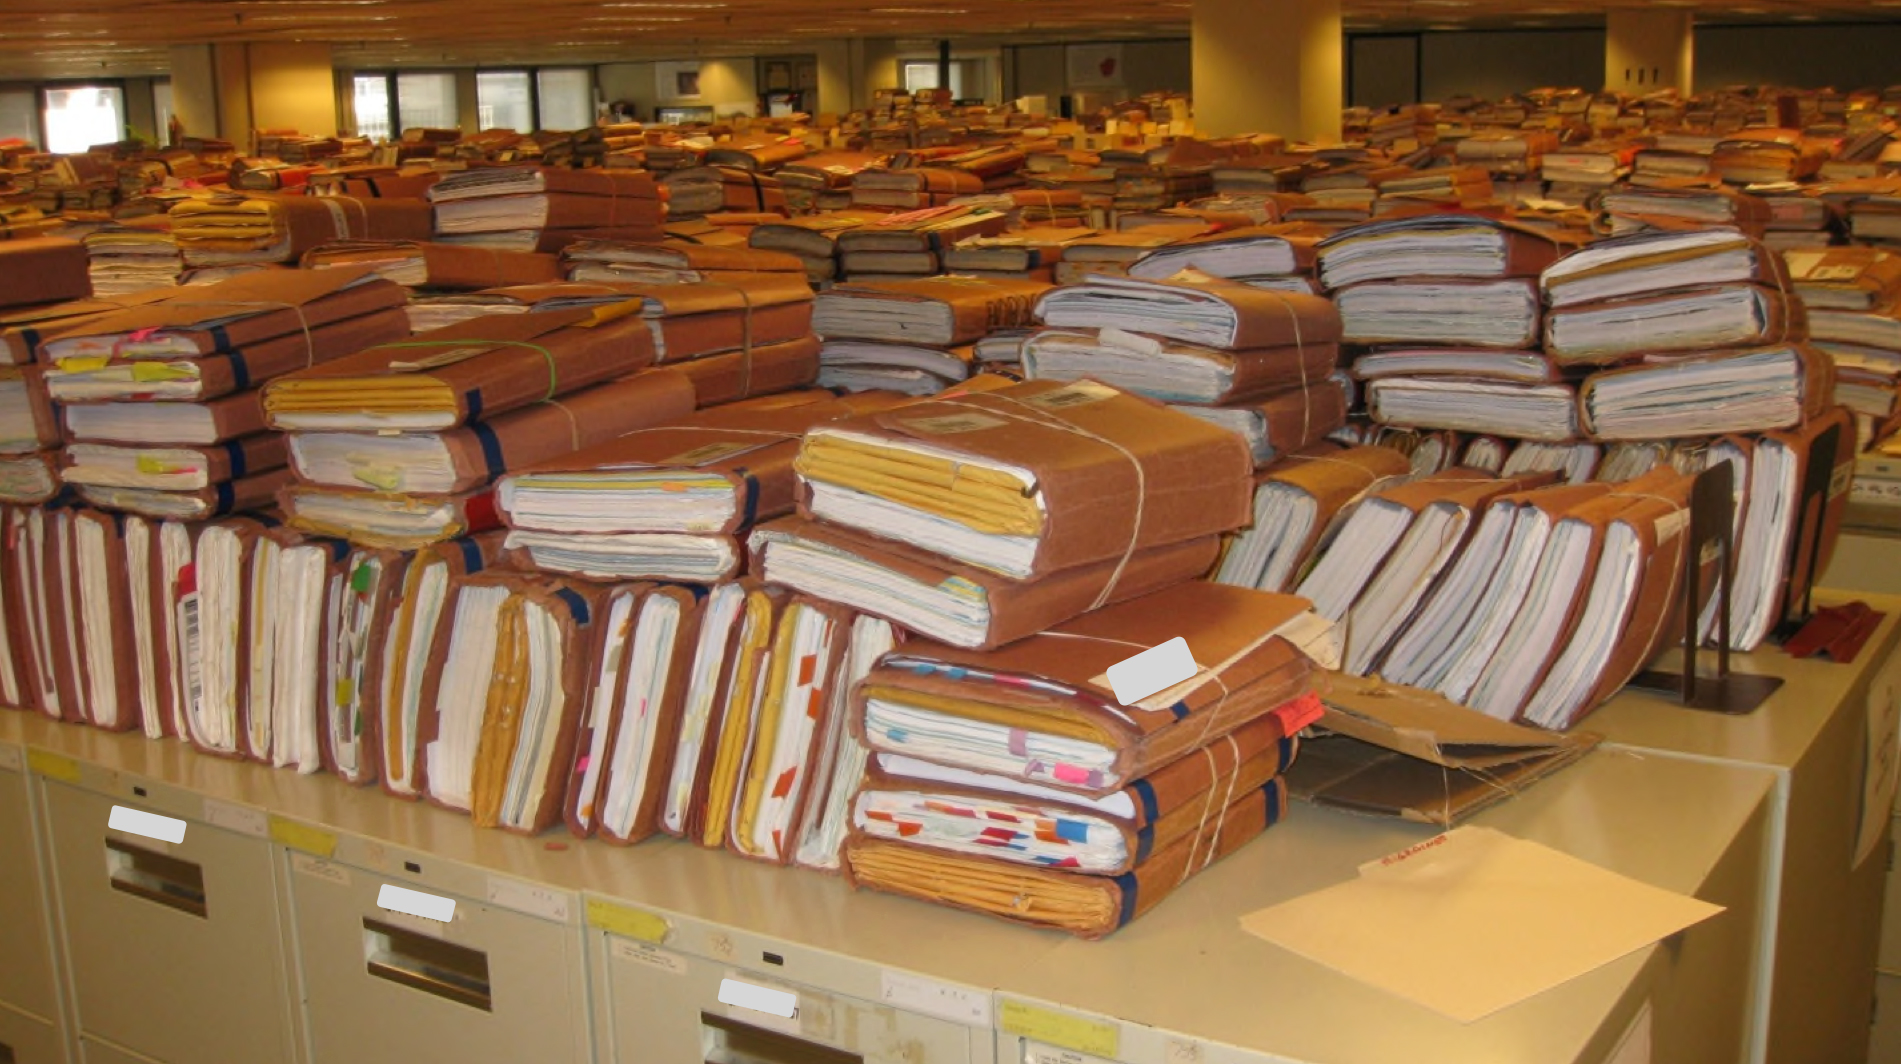
\includegraphics[width=0.8\textwidth]{basementfiles.jpg}}

\begin{frame}{Manifests}
 We can take this one step further, be tying together various swarm assets under a new root-hash by generating a new tree: A \textbf{Manifest}\\
 \begin{block}{A Swarm Manifest...}
  ...is a Merkle tree whose leaves are root-hashes of other swarm assets (files, collections, manifests, chunks...)
 \end{block}
 The only difference between this and the chunk-tree of a file, is that it is not balanced and has metadata.
\end{frame}

\begin{frame}
 For example, \uncover<2->{the Swarm landing page
 \begin{center}
  \texttt{swarm-gateways.net/bzz:/swarm/}
 \end{center}
 }
 \end{frame}

\begin{frame}
 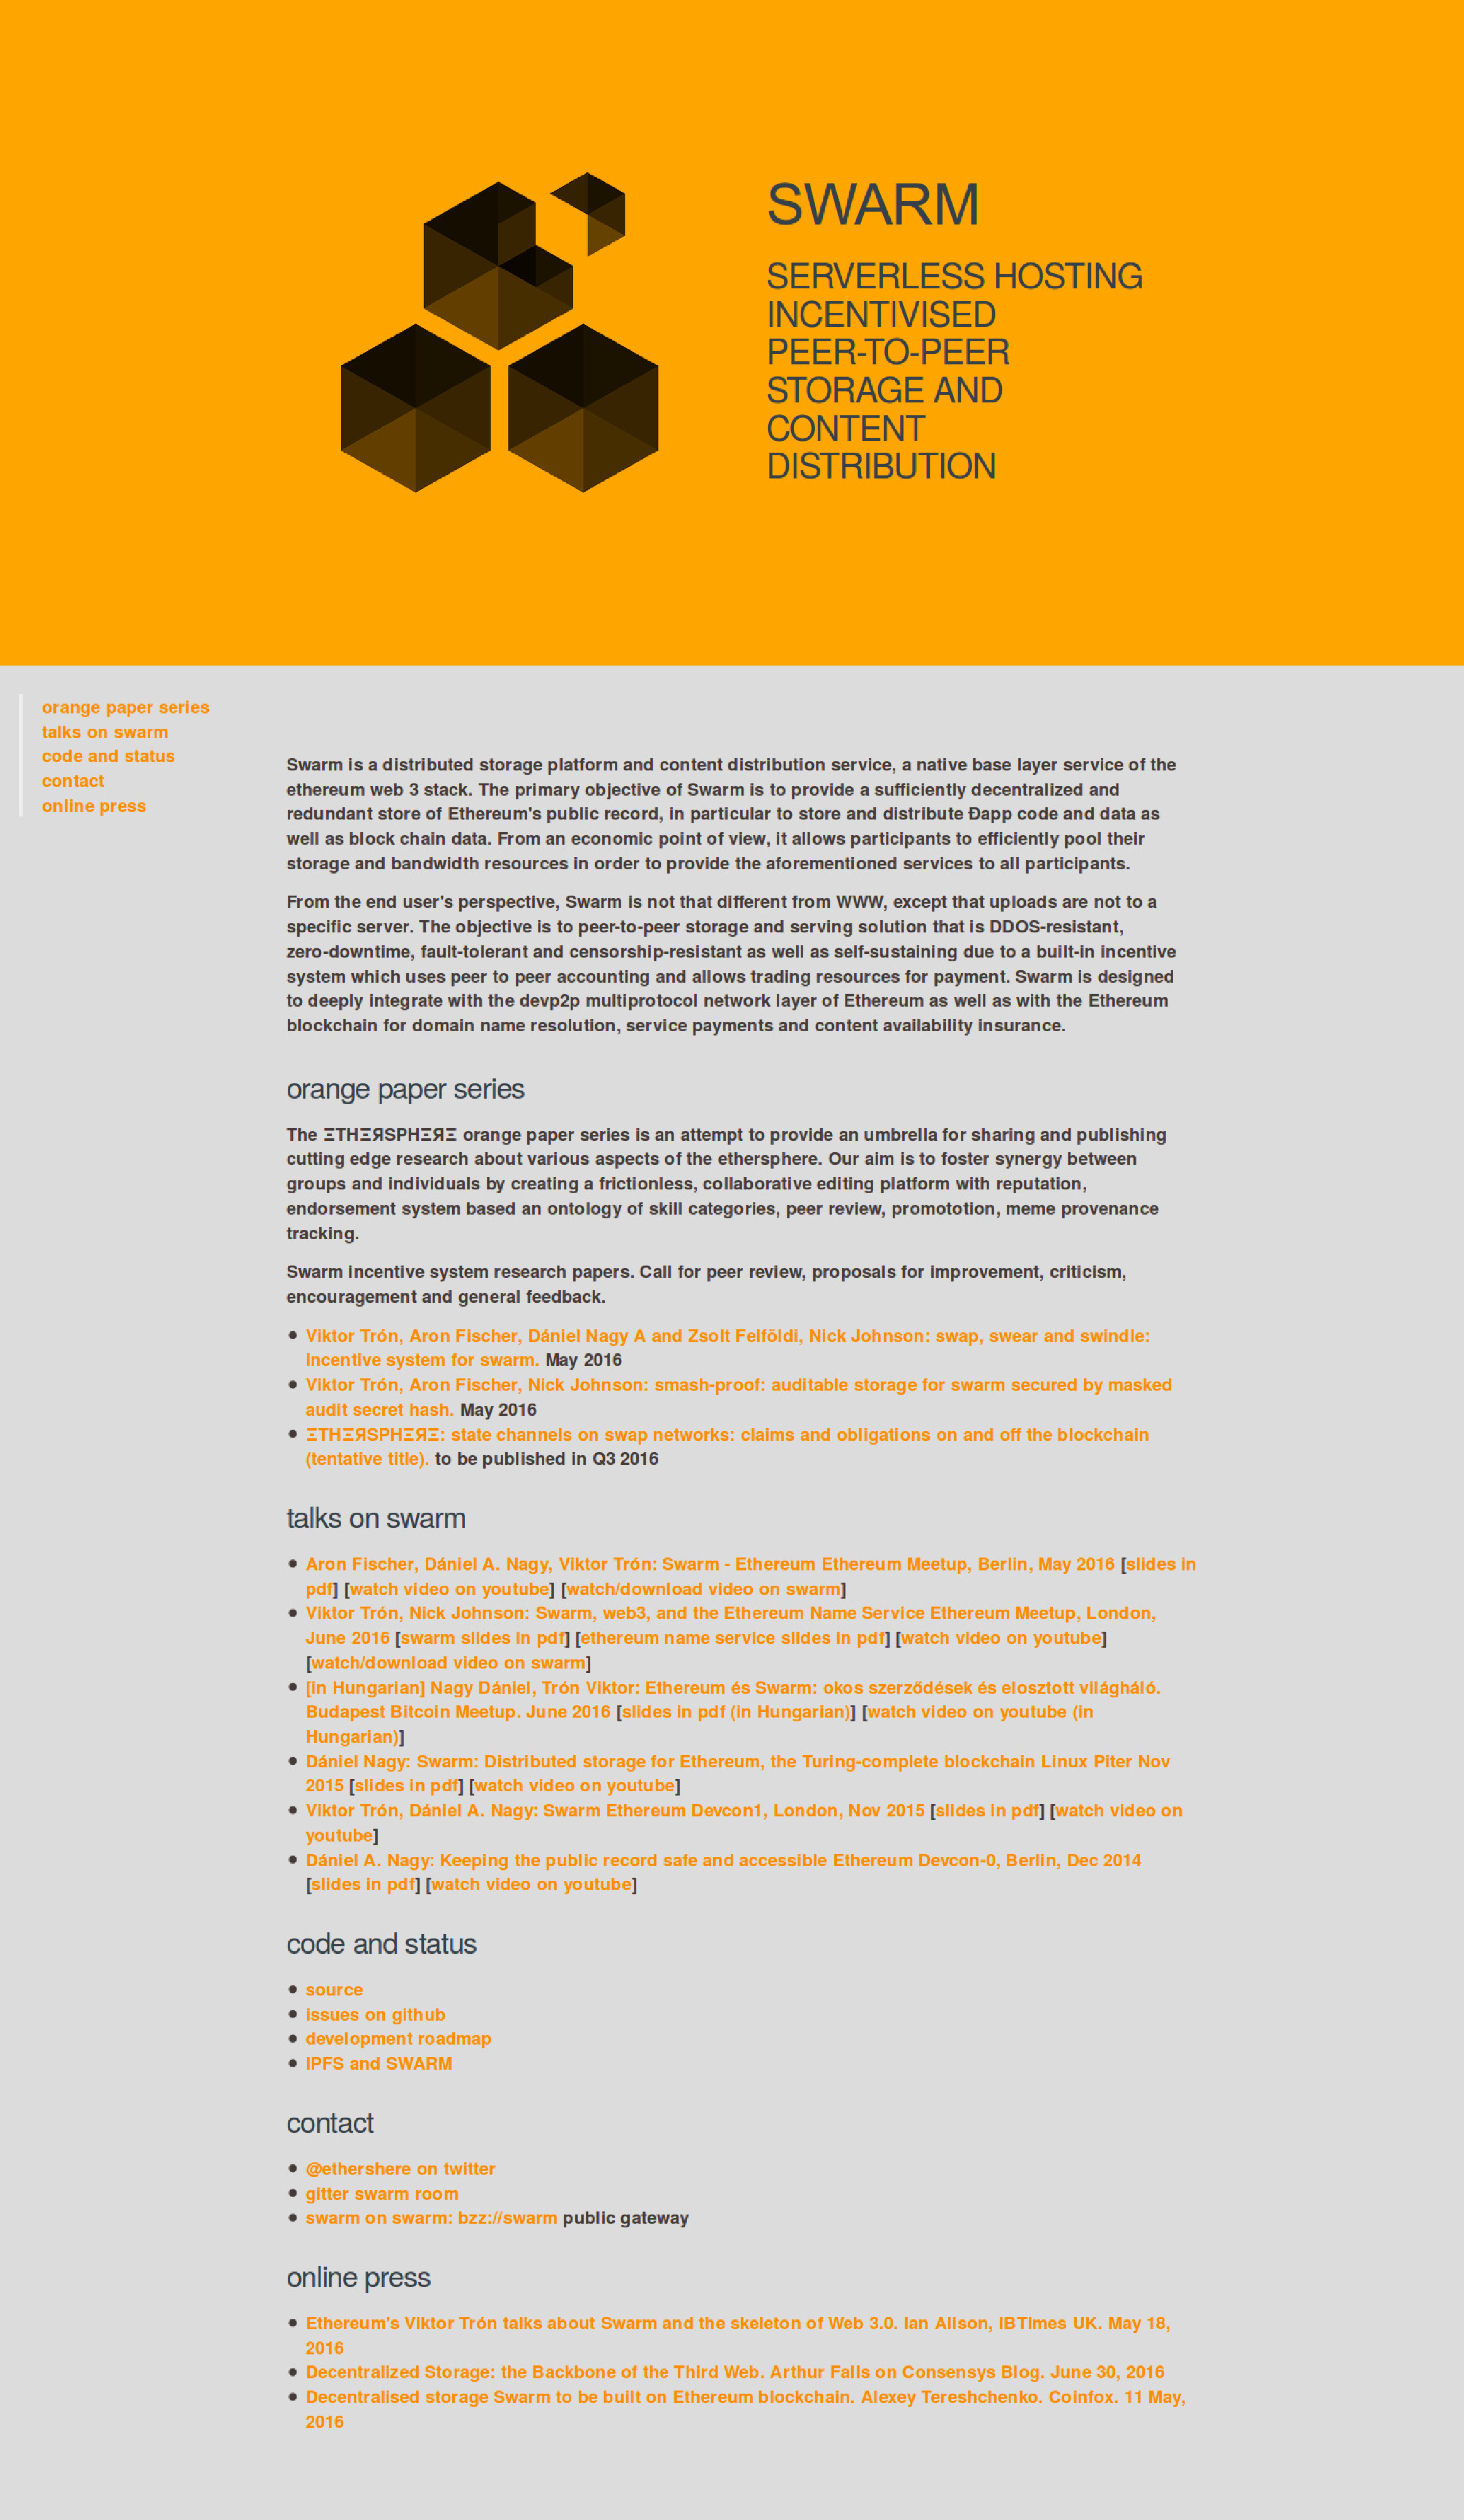
\includegraphics[width=0.8\textwidth]{devcon-swarmsite.pdf}
\end{frame}

\begin{frame}[fragile]
\frametitle{Manifests}
 ...is loaded from this 4-entry manifest:\\
\tiny
\begin{semiverbatim}
\{"entries":[\{
"path":"Swarm_files/",
"hash":"0294e48456a49fe7c02162c83b068075ff9ae6aaafb46439dba32da7de548379",
"contentType":"application/bzz-manifest+json",
"status":0\},
\{"path":"ethersphere/orange-papers/"...
\{"path":"i"...
\{"path":"talks/"...
\{"path":"",
"hash":"6fac0b0c1f118f7f383792c0f01c80d1b2dc94f0e166d62ff4f999a926e9d94a",
"contentType":"text/html;charset=utf-8","status":0\}]\}\end{semiverbatim}
\uncover<2->{\small
 Manifests translate a URL path into swarm hashes (URL defines manifest merkle-tree traversal).\\[2mm]
 When combined with the Ethereum Name Service (ENS) to register a name for the manifest's own root hash, we can \textbf{serve any and all swarm data directly to your browser using human readable names}.
}
\end{frame}

 \begin{frame}{Example: Swarm File Manager}
  With manifests, you can navigate swarm just like you would navigate your own filesystem.\\
  \uncover<2->{Let us open the swarm landing page in the swarm file manager:\\}
  \uncover<3->{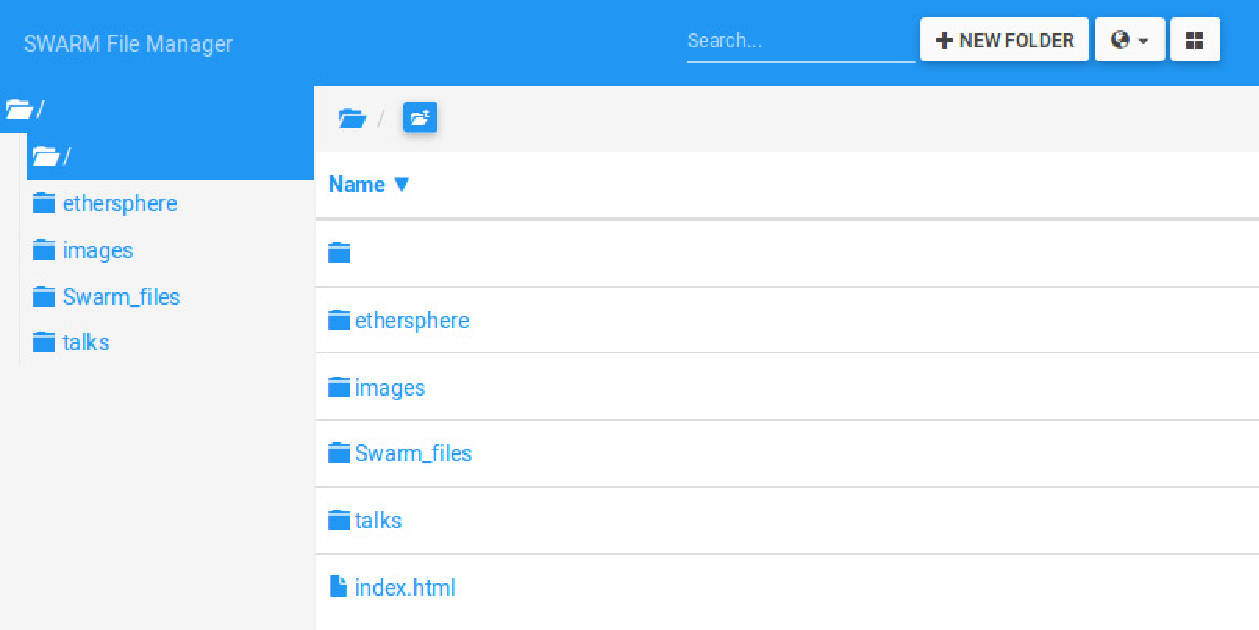
\includegraphics[width=11cm]{devcon-swarmfilemanager.pdf}}
 \end{frame}

\begin{frame}{}
\begin{block}{manifests}
\begin{itemize}
 \item only root hashes need to be registered (ENS) on blockchain
 \item site is integrity protected
 \item two-way translation possible from directories to routes on the domain
  \end{itemize}
\end{block}
\begin{block}{manifests enable}
  \begin{itemize}
   \item filesystem API
   \item Dropbox, rsync, ...
   \item filesystem driver (FUSE)
  \end{itemize}
  \end{block}
\end{frame}


\begin{frame}{}
\begin{block}{extend manifests with metadata}
\begin{itemize}
      \item http headers
      \item copyright information
      \item access control
      \item payment triggers
      \item auto-play continuation
      \item subscription information
      \item database layout info
\end{itemize}
\end{block}


\end{frame}



\begin{frame}
\setbeamercovered{transparent}% Dim out "inactive" elements
\begin{overlayarea}{\textwidth}{10cm}
\begin{block}{How are database services organised?}
\begin{itemize}
\item<1-> structure  - manifests
\item<2-> security - blockchain proofs
\item<3-> scalability - off-chain computation
\item<4-> sustainability - incentives
\end{itemize}
\end{block}
\begin{block}{How?}
\begin{itemize}
\only<1>{
\item manifests implement key-value store (Patricia Merkle Trie as oppose to traditional DHT)
\item supports various indexes and iteration (range queries)
\item conventions db table layouts in manifest metadata
\item table and index roots anchored in Ethereum Name Service
}
\only<2>{
\item verifiable on the blockchain by challange
\item verifiable authentication, record updates and notifications
\item verifiable indexes, query resolution
}
\only<3>
{
\item sql resolver (this reql of rethinkdb) sitting on top
\item parallel processes walk the indexes and merge results
\item index updates, derivative data (full text search indexes, aggregate statistics) supplied by a computational market
\item query caching and accelerated retrieval for real-time low latency experience supplied by specialised nodes
}
\only<4>
{
\item due to verifiable computations (truebit, ewasm), \textit{swap, swear and swindle} is applicable
\item positive and negative incentivisation
\item secondary market for compensatory insurance
}
\end{itemize}
\end{block}
\end{overlayarea}
\end{frame}

\plainblockslide{}{\textsc{sword}: \textbf{S}tate \textbf{W}ith \textbf{O}n-demand \textbf{R}etrieval of \textbf{D}ata}

\begin{frame}
\begin{block}{can we put the ethereum blockchain and state on swarm}
\begin{itemize}
 \item light client - flexible transition from remote, light, full and archival nodes
 \item solves the scalability problem of too big state data, receipts, contract storage, fast syncing
 \item decentralised blockchain explorer
\end{itemize}
\end{block}
\end{frame}



\end{section}
\end{document}
